\documentclass{article}

\usepackage{graphicx}
\usepackage{tikz}
\usetikzlibrary{automata,positioning}

\begin{document}

Here the modelling is presented as described by Kendall. We consider a small element of time $dt$.


If $dt$ is small enough, an evolution of the system by a jump larger than one is highly unlikely and can be neglected.

The following possible evolutions are of interest: $N(t+dt)=N(t)+1$, $N(t+dt)=N(t)-1$, and $N(t+dt)=N(t)$.\\

The probability for the event $N(t+dt)=N(t)+1$ is: $\lambda \times N(t) \times \mathrm{d}t+o(dt)$ \\

The probability for the event $N(t+dt)=N(t)-1$ is: $\mu \times N(t) \times \mathrm{d}t +o(\mathrm{d}t)$ \\

The probability for the event $N(t+dt)=N(t)$ is: $1 - (\mu+\lambda) \times N(t) \times \mathrm{d}t +o(\mathrm{d}t)$ \\



\begin{figure}[here!] 

\centering

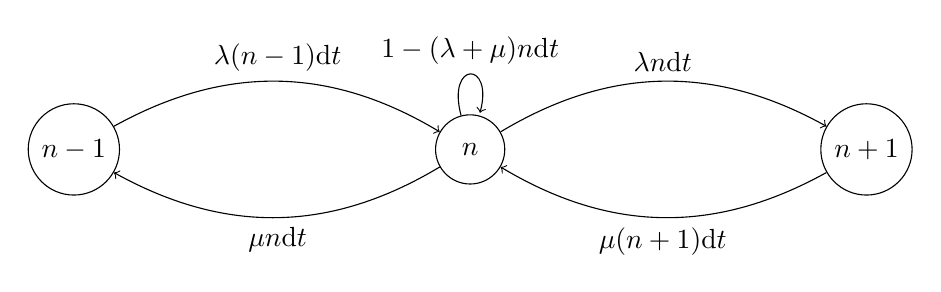
\begin{tikzpicture}

\node[state] (0) {$n-1$};

\node[state,right= 4cm of 0] (1) {$n$};

\node[state,right= 4cm of 1] (2) {$n+1$};

\draw[]     

   % From zero to zero

  %(0) edge[loop above] node {$1-(\lambda+\mu)(n-1)dt $}   (0)

  % From one to one

  (1) edge[loop above] node {$1-(\lambda+\mu) n \mathrm{d}t $}   (1)

  % From two to two

 % (2) edge[loop above] node {$1-(\lambda+\mu)(n+1)dt $}   (2)

  % From zero to one

  (0) edge[->,bend left] node[anchor=south] {$\lambda(n-1)\mathrm{d}t $}   (1)     

  % From one to zero 

  (1) edge[->,bend left] node[anchor=north] {$\mu n \mathrm{d}t $}   (0)  

  

  % From one to two 

  (1) edge[->,bend left] node[anchor=south] {$\lambda n \mathrm{d}t$}   (2) 

  

  % From two to one 

  (2) edge[->,bend left] node[anchor=north] {$\mu (n+1) \mathrm{d}t$ }   (1) 

  

    

;

\end{tikzpicture} 

\caption{Time continuous Markov model; the figure represents a system that has $n$ $(n\ge 1)$ species at time $t$ and  indicates the possible states at time $t+\mathrm{d}t$ as well as the probabilities associated with these transitions.} \label{fig:markov}

\end{figure}




$P(N(t)=n)$, the probability of n species at time t, will be noted $P_n(t)$.\\


The following system of differential equations is deduced from these previous observations:

\begin{align}

&\frac{\mathrm{d}P_n(t)}{\mathrm{d}t}=P_{n-1}(t)\lambda(n-1)+P_{n+1}(t)\mu(n+1)-(\lambda+\mu)P_n(t) n \; ; \; n\ge 1 \\

&\frac{\mathrm{d}P_0(t)}{\mathrm{d}t}= \mu P_1(t)

\end{align}

An initial condition has also to be taken into account: the number of species at $t=0$, $n_0$ has to be known for the system being solved. We have then $P_{n_0}(0)=1$.\\

A birth rate, a death rate and an initial number of species are sufficient for describing a birth death process. 
Of course, in a stochastic framework the evolution of the process is not deterministic but it can be characterized by the 
expectation and the variance of the number of species over time. A birth death process will be noted $(\lambda,\mu,n_0)$.





\end{document}



 
